Die hier zu entwickelnde Anwendung dient zum Anlegen und Verwalten von Aufgaben der Nutzer. Somit löst sie die sogenannte, analoge \textit{To-Do-Liste} ab. Dabei hat die Anwendung (und somit auch die Studienarbeit) keinen Anspruch auf Innovationsdarbietung. Die Begründung der dieses speziellen Entwicklungsbeispiels liegt darin, dass eine To-Do-Listen-Anwendung ein großes Spektrum von Funktionen abbilden kann. Dieses Spektrum reicht von grundlegenden Funktionen (bspw. dem bloßen Anlegen von Aufgaben) bis zu komplexeren Inhalten (bspw. automatischen Push-Notifications über unerledigte oder überfällige Aufgaben). Diese design- und architekturbedingenden Entscheidungen werden im Folgenden definiert und näher beschrieben.

Die Beschreibung der Architektur einer zu entwickelnden Applikation ist eine maßgebende Disziplin im Software-Engineering-Prozess. Dieser Prozess geschieht vor Beginn der Implementierung und ermöglicht, bezogen auf den Umfang dieser Studienarbeit, die Vergleichbarkeit der Applikation hinsichtlich der relevanten Entwicklungsplattformen. Der Umfang sämtlicher Software-Engineering-Prozesse wird grundsätzlich in großen Entwicklerteams praktiziert. Diese gehen der Entwicklung meist komplexer und skalierbarer Anwendungen nach. Im Vergleich dazu ist die hier zu entwickelnde Mobilanwendung lediglich Mittel zum Zweck für die Beantwortung der Forschungsfrage. Das Entwicklungsteam der To-Do-Anwendung besteht aus zwei Personen, welche sich im Rahmen dieser Arbeit autark mit unterschiedlichen Entwicklungsplattformen beschäftigen.

Dies sorgt dafür, dass sich lediglich eine abgespeckte Form des Software-Engineering auf dieses Projekt anwenden lässt. Konkret bedeutet dies, dass keine spezifischen Aussagen über den Software-Prozess bzw. über das Entwicklungsmodell (Wasserfall-Modell, iteratives Modell, etc.) gemacht werden. Dies würde sich hinsichtlich des verhältnismäßig geringen Entwicklungs- und Wartungsaufwands der App kontraproduktiv auf die Zielorientierung auswirken. Umso wichtiger ist die Definition funktionaler sowie nicht-funktionaler Anforderungen, welche daraufhin näher erläutert und spezifiziert werden. Auch die Interaktion zwischen Nutzer und Anwendung muss für eine vergleichende Entwicklung definiert werden. Die zeitlichen und komponentenabhängigen Abläufe innerhalb der App gehören ebenfalls zu den Bestandteilen der Architektur. Letztere beiden Punkte werden im Rahmen des sog. \textit{Systems Modelling} definiert. Darüber hinaus werden auch optische Aspekte und Verhaltensweisen des \ac{ui} abgegrenzt.

\section{Anforderungsdefinition} \label{sec:3-anfoderungen}
Die Funktionalität der Anwendung wird zunächst über die Anforderungsdefinition näher beschrieben. Diese kann auf allgemeine Funktionsweisen der App (nicht-funktionale Anforderungen), sowie auf spezifische, technische Charakteristika abgegrenzter Bereiche der Anwendung (funktionale Anforderungen). Grundsätzlich gilt es, nicht-funktionale Anforderungen im Laufe der Anforderungsdefinition in meist mehrere funktionale Anforderungen zu überführen, da diese qualifizierbarer sowie quantifizierbarer Natur sind und somit ebenfalls für eine bessere Vergleichbarkeit der zu entstehenden Anwendungen beitragen könnten.

\subsection{Nicht-Funktionale Anforderungen}
Die folgenden nicht-funktionalen Anforderungen beziehen sich auf Teile der Anwendung, welche jedoch abstrakter Natur sind, weswegen sie zunächst zu nicht-funktionalen Anforderungen gezählt werden müssen. Aufgrund der Formulierung werden diese Anforderungen auch als \textit{Nutzeranforderungen} (engl. \textit{User Requirements}) bezeichnet und stehen den spezifischeren, technisch versierteren \textit{Systemanforderungen} (engl. \textit{System Requirements}) gegenüber.
\begin{description}
    \item[Anlegen, Auflisten, Bearbeiten und Löschen von Aufgaben] Die Anwendung ermöglicht es, Aufgaben hinzuzufügen. Die hinzugefügten Aufgaben werden aufgelistet. Bei Bedarf soll der Inhalt der Aufgabe nachträglich abgeändert werden können. Ebenfalls ist es möglich, die Aufgabe aus der Ansicht innerhalb der Anwendung zu entfernen.
    \item[Aufgaben bestehen nach Neustart der Anwendung bei] Wird die Applikation (gewollt und ungewollt) neu gestartet, bildet sie nach Neustart dieselben Aufgaben und Einstellungen wie zuvor ab.
    \item[Priorisierung der Aufgaben möglich] Bei Bedarf ist es möglich, einer bestimmten Aufgabe einen gesonderten Stellenwert zuzuweisen.
    \item[Benachrichtigungen über nicht-erledigte und überfällige Aufgaben] Der Nutzer wird unabhängig vom Status der Applikation oder des Smartphones (d.h. online/offline, geöffnet, im Hintergrund oder geschlossen bzw. gesperrt oder entsperrt) über nicht-erledigte und überfällige Aufgaben benachrichtigt.
\end{description}
Neben dieser Art der nicht-funktionalen Anforderungen koexisitieren jene, welche zwar ebenfalls abstrakt und allgemein gehalten sind, jedoch keinen Bedarf resp. keine Möglichkeit zur weiteren Spezifizierung an dieser Stelle des Prozesses aufweisen.
\begin{description}
    \item[Bereitstellung der Anwendung für mehrere Plattformen] Die Anwendung ist nicht nur auf einer Plattform verfügbar, sondern kann auf Geräten unterschiedlicher Betriebssysteme installiert und verwendet werden.
    \item[Aussehen und Verhalten sind deckungsgleich] Unabhängig davon, welche Plattform genutzt wird, ist die Interaktion zwischen dem Nutzer und der Anwendung annähernd identisch. Davon ausgenommen sind Aspekte, welche auf der entsprechenden Plattform nicht oder nur mit unverhältnismäßigem Aufwand erreicht werden können.
    \item[zeiteffizienter Entwicklungsprozess] Um auch einen entwicklungstechnischen Vergleich ziehen zu können, soll die Anwendung in einer dem Projekt angemessenen Zeit vollständig entwickelt werden können.
\end{description}
Die Problematik nicht-funktionaler Anforderungen im Bezug auf realistisch zu betrachtende Entwicklungsprojekte kann hier interpretiert werden. Vor allem bei eher unerfahrenen Entwicklern (zu welchen sich das Entwicklerteam dieses Projektes zu zählen erlaubt) sind bestimmte Tendenzen unklar. Dazu gehören bspw. das Bewusstsein über die Realisierbarkeit bestimmter Komponenten sowie die zeitliche Aufwandseinschätzung. Diese Störfaktoren werden im Laufe der Arbeit versucht, entkräftet zu werden und sind in die Evaluation der Forschungsfrage kritisch einzubeziehen.

\subsection{Funktionale Anforderungen}
Nichtsdestotrotz ist die Spezifizierung der in Sektion 3.1.1 eingangs definierten nicht-funtionalen Anforderungen noch ausstehend. Zur Unterstützung der Lesbarkeit werden diese in Reihenfolge der nicht-funktionalen Anforderungen abgehandelt.

\begin{description}
    \item[Bereitstellung klassischer \acs{crud}-Operationen] Sog. \textit{\ac{crud}}-Operationen greifen auf das Datenmodell der Anwendung zu. Diese erlauben die Manipulation der Daten auf Basis der gewünschten Operation. Diese Operationen sind unabhängig voneinander zu definieren und sinnvoll in den Verwendungsprozess der App einzubauen. Man spricht hier auch von sog. \ac{crud}-\textit{Endpoints}, welche vereinfacht als statische Funktionen beschrieben werden können.
    \item[Listendarstellung] Die Aufgaben sollen grundsätzlich in einer sortierten Liste dargestellt werden. Die Liste besteht aus individuellen Elementen, welche jeweils eine Aufgabe darstellen. Jene \ac{crud}-Operationen, welche speziell auf eine bestimmte Aufgabe angewandt werden sollen, finden ihre Aktivierung ebenfalls über ihre entsprechenden Elemente.
    \item[Bereitstellung eines Persistent Services] Bei Ausführen der zuvor definierten \ac{crud}-Operationen werden die Daten nicht nur in den flüchtigen Arbeitsspeicher des Smartphones geschrieben, sondern zugleich auch auf einen der Applikation zugewiesenen Festspeicher. Diese idealisierte Datenbank gleicht dem Datenmodell für die \ac{crud}-Operationen und wird somit bei jeder Ausführung dieser aktualisiert bzw. beansprucht.
    \item[Definition einer Hierarchie für Aufgaben] Eine hierarchische Struktur der Daten soll ermöglichen, bestimmte Aufgaben seitens der Anwendung anders zu behandeln als andere. Durch das Setzen eines sog. \textit{Flags} können die Aufgaben entsprechend der Hierarchiestruktur bestimmte Zustände übergeben bekommen, konkret eine hervorgehobene optische Darstellung innerhalb der \ac{ui} sowie die Präsentation an Anfang der Liste (Eingriff in die Sortierung der Aufgaben)
\end{description}


Streng genommen sind funktionale Anforderungen sehr granular zu definieren. Da es sich hier jedoch um eine wissenschaftliche Arbeit handelt, und nicht um eine Entwicklerdokumentation, wird auf eine detaillierte Beschreibung verzichtet. Viel eher soll die nächste Sektion die genaue, weiterhin plattformunabhängige Umsetzung dieser Anforderungen eräutern, welche als Maßgabe für die spätere Entwicklung der Applikation dienen soll. \\\

Unabhängig von der Plattform wird zunächst ein allgemeines, während der individuellen Entwicklungsphase zu spezifizierendes Grundgerüst der Funktionalität definiert. Bei einer To-Do-Applikation besteht dieses grundsätzlich aus zwei Komponenten. Die idealisierte \textit{Datenbank} ermöglicht persistente Speicherung der angelegten To-Do-Einträge. Diese ist mit verschiedenen \ac{crud}-Funktionen direkt an das \ac{ui} angebunden und ermöglicht somit die Manipulation der Einträge.

\section{Speicherung der Daten} \label{sec:3-speicherung-daten}
Die Datenbank muss auf eine Weise angelegt werden, dass ihre Daten (d.\ h. To-Do-Einträge) einem bestimmten Schema folgen. Konkret bedeutet dies folgende Attribute für die Entität \texttt{ToDo}:

% TODO Tabellarische Darstellung der Attribute
\begin{itemize}
	\item[\texttt{id}] (alpha-)numerische Zeichenfolge, welche einen Eintrag eindeutig erkennbar macht (String)
	\item[\texttt{text}] anzuzeigender Text, welcher den eigentlichen Eintrag darstellt und beschreibt (String)
	\item[\texttt{done}] Status über die Erledigung des entsprechenden Eintrages (Bool'scher Wert)
	\item[\texttt{priority}] Status über die Priorität des entsprechenden Eintrages (Bool'scher Wert)
\end{itemize}

% TODO Beispiel der idealisierten Datenbankeinträge
Unabhängig von der individuellen Architektur der jeweiligen Apps folgt dieses triviale Schema dem Konzept relationaler Datenbanken und könnte somit in einer einfachen Tabelle dargestellt werden.

Um auf die Datenbank zugreifen zu können, muss diese mit entsprechenden Funktionen ausgestattet werden. Neben dem bloßen Erstellen von Einträgen, müssen diese abgegriffen (engl. \textit{fetch}) sowie bearbeitet und gelöscht werden können. Die beiden letztgenanten Funktionen haben bei Ausführung nur Einfluss auf einen durch den*die Nutzer*in ausgewählten Eintrag. Somit müssen diese Funktionen das \textit{Objekt} des entsprechenden Eintrages übergeben bekommen. Weiterhin gliedert sich die Bearbeitung von Einträgen in drei Teilfunktionen auf, nämlich dem Ändern des \texttt{done}- oder \texttt{priority}-Attributes sowie dem Ändern des beschreibenden Textes des Eintrags.

Da die Ausführung sowie Umsetzung dieser Operationen mit der \ac{ui} Hand in Hand geht, wird die Definition dieser vorgezogen.


\section{Benutzeroberfläche (\acs{ui})} \label{sec:3-ui}
Die Benutzeroberfläche einer solch einfachen To-Do-Anwendung besteht aus einer Ansicht. Diese Ansicht lässt sich hierarchisch definieren. Die oberste Ebene dieser Hierarchie bildet der hier sog. \textit{App-Container}. Anders als in aufwändigeren Applikationen kann dieser hier mit der Ansicht gleichgesetzt werden, da keine weiteren Ansichten existieren. Dieser Container beherbergt eine Listenansicht, welche für die Darstellung und Interaktion mit den bereits vorhandenen Einträgen zuständig ist. Für das Erstellen der Einträge steht ein separates Text(eingabe)feld zur Verfügung, sowie ein \textit{Button} zur Bestätigung der Eingabe.

Die Listenansicht besteht nun aus mehreren Listeneinträgen (im Folgenden \texttt{Zellen} genannt). Eine Zelle ist für die Darstellung und Interaktion für genau einen To-Do-Eintrag zuständig. Um dies zu ermöglichen, besitzt jede Zelle, neben eines Textfeldes zum Anzeigen des To-Do-Textes, weitere Buttons zum Setzen der Priorität und des Status sowie zum Löschen des Eintrages. Während der Button, welcher für das Entfernen des Eintrages verwendet wird (dargestellt durch ein Kreuz, statischer optischer Natur ist (d.\ h., er ändert nach einem Tippen sein Aussehen nicht), untermalen die Buttons der To-Do-Zustände die gewählten Einstellungen durch ihr Aussehen. Der Button für Priorisierung, welcher durch ein Sternsymbol dargestellt wird, ist bei aktiver Priorisierung gefüllt. Ist dies nicht der Fall, so ist lediglich der Umriss des Symbols zu erkennen. Gleiches gilt für den Button, welcher anzeigt, ob der Eintrag bereits erledigt ist, dargestellt durch ein Häkchen inmitten eines Kreises.

Die beschriebenen, visuellen Eigenschaften lassen sich nun in einem sog. \textit{Wireframe} zusammenfassen, welches gleichzeitig die optische Grundlage der Entwicklung darstellen wird. Dies ist vor allem aufgrund der unterschiedlichen Entwicklungsplattformen von Relevanz, da das Einhalten bestimmter Standards der entsprechenden Plattformen dafür sorgen könnte, dass der letztendliche Vergleich beider Applikationen hohe Differenzen aufweist.

\begin{figure}[h!]
	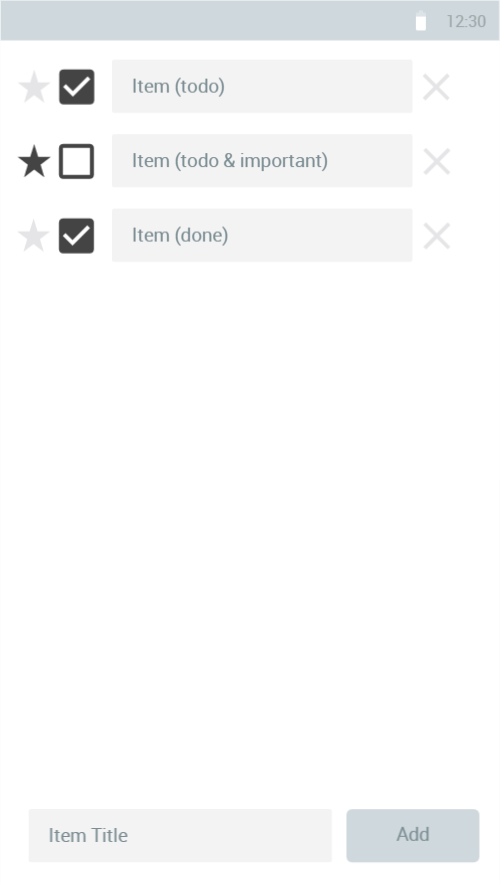
\includegraphics[scale=0.5]{img/wireframe.png}
	\centering
	\caption{Wireframe}
	\label{fig:wireframe}
\end{figure}

Eine Besonderheit in der Darstellung lässt sich innerhalb der priorisierten Elemente finden. Um diese weiter hervorzuheben, werden diese an den Anfang der Liste gesetzt. Es entstehen somit zwei Teillisten, welche sich jedoch in derselben Listenansicht befinden. Wird nun ein zuvor nicht-priorisierter Eintrag priorisiert, so wechselt dieser seine Position ans Ende der Liste mit den bereits priorisierten Einträgen (bzw. wird oberhalb der ersten nicht-priorisierten Elements platziert). Alle Einträge zwischen der alten und der neuen Position des gerade betrachteten Eintrags werden um eine Listenposition nach unten verschoben. Bei Entfernen der Priorisierung wird das entsprechende Element nun nicht an seine ursprüngliche Position vor der Priorisierung, sondern an den Anfang der nicht-priorisierten Liste verschoben. Entfernt man also bspw. die Priorisierung des letzten Elements in der priorisierten Liste, ändert sich die Reihenfolge nicht. Dieses Verhalten kann vereinfacht in der untenstehenden Abbildung dargestellt werden.

Grundsätzlich werden alle Einträge in der Reihenfolge dargestellt, wie sie angelegt wurden, mit den eben beschriebenen Ausnahmen.


\subsection{Farbliche Darstellung}
Um ebenfalls für farbliche Konsistenz zu sorgen, werden die beschriebenen Elemente auf Basis der folgenden Tabelle in ihrem Erscheinungsbild konfiguriert:

\begin{table}[h!]
	\centering
	\begin{tabular}{ |c|c|c|}
		\hline
		\textbf{Bezeichnung} & \textbf{HEX-Code} & \textbf{Beispiel}\\
		\hline
		
		
		\hline
		\multicolumn{3}{|c|}{\textbf{Allgemeines}}\\
		\hline
		Hintergrund & \texttt{\#F2F2F2} &\cellcolor[HTML]{F2F2F2}\\
		\hline
		Schriftfarbe & \texttt{\#8C8C8C} &\cellcolor[HTML]{8C8C8C}\\
		\hline
		
		
		\hline
		\multicolumn{3}{|c|}{\textbf{Bedienelemente}}\\
		\hline
		Hintergrund für inaktive Bedienelemente & \texttt{\#CECECE} &\cellcolor[HTML]{CECECE}\\
		\hline
		Checkbox (checked) Hintergrund & \texttt{\#1A66FF} &\cellcolor[HTML]{1A66FF}\\
		\hline
		Schriftfarbe der Checkbox (checked) & \texttt{\#FFFFFF} &\cellcolor[HTML]{FFFFFF}\\
		\hline
	\end{tabular}
	\caption{Farbtabelle} \label{tab:farbtabelle}
\end{table}


% Spaß mit Activity-Diagrammen!
\section{Nutzungszyklus} \label{sec:3-nutzungszyklus}
Der Nutzer öffnet die Anwendung. Beim Laden der Ansicht wird eine Datenbank-Funktion ausgeführt, um bereits existierende Einträge zu laden und ihre entsprechenden Beschreibungen samt weiteren Attributen in die einzelnen Zellen der Listenansicht zu laden. 

Der Nutzer möchte einen neuen To-Do-Eintrag erstellen. Dafür wird ein beschreibender Text in das Texteingabefeld am unteren Rand der Ansicht geschrieben. Um einen neuen Eintrag zu erstellen, wird ein beschreibender Text in das Texteingabefeld am unteren Rand der Ansicht geschrieben. Mit der Bestätigung über den \texttt{+}-Button wird ein neuer Eintrag in die Datenbank aufgefordert, wobei das \texttt{text}-Attribut mit dem zuvor gewählten Text aus dem Eingabefeld gefüllt wird. Die Zeichenfolge der \texttt{id} wird automatisch und zufallsbasiert generiert, \texttt{done} sowie \texttt{priority} standardmäßig auf \texttt{false} gesetzt. Der neue Eintrag wird unter den bereits vorhandenen Einträgen angefügt. Stern- sowie Häkchen-Symbol werden lediglich über ihre Kontur kenntlich gemacht.

Der Nutzer möchte den Test eines Eintrages ändern. Durch direktes Tippen auf den dargestellten Text in einer Zelle wird dies ermöglicht. Es erscheint ein Cursor, welcher ebenfalls Tastatur- und Berührgesten innerhalb dieses Feldes ermöglicht. Nach bestätigter Änderung über das Verlassen des Textfeldes (d.\ h. dem Tippen auf eine andere Stelle innerhalb der Ansicht) wird erneut eine Datenbank-Funktion ausgeführt. Diese bekommt das \texttt{ToDo}-Objekt übergeben und ersetzt den bestehenden Inhalt des \texttt{text}-Attributes mit dem nun geänderten.

Der Nutzer möchte den zuvor erstellten Eintrag priorisieren. Tippt dieser auf das Stern-Symbol, wird dieses mit der zuvor definierten Farbe gefüllt. Gleichzeitig bewegt sich das priorisierte Element an das Ende der Teilliste mit priorisierten Einträgen. Eine Datenbank-Funktion wird aufgerufen, welche den \texttt{priority}-Wert des übergebenen Objekts von \texttt{false} auf \texttt{true} setzt.

Der Nutzer möchte den zuvor priorisierten Eintrag als abgeschlossen markieren. Tippt dieser auf das Häkchen-Symbol wird dieses mit der zuvor definierten Farbe gefüllt. Eine Datenbank-Funktion wird aufgerufen, welche den \texttt{done}-Wert des übergebenen Objekts von \texttt{false} auf \texttt{true} setzt.

Der Nutzer möchte den zuvor als abgeschlossenen Eintrag aus der Liste der priorisierten Einträge entfernen. Tippt dieser auf das Stern-Symbol, wird dessen Füllung entfernt. Gleichzeitig bewegt sich das Element an den Anfang der Teilliste mit nicht-priorisierten Einträgen. Die zuvor ausgeführte Datenbank-Funktion wird erneut aufgerufen, welche den \texttt{priority}-Wert des übergebenen Objekts von \texttt{true} nun wieder auf \texttt{false} setzt.

Der Nutzer möchte den Eintrag abschließend entfernen. Tipps dieser auf das Kreuz-Symbol, wird der Eintrag aus der Liste entfernt. Die Elemente unterhalb des gelöschten Eintrags verschieben sich um jeweils eine Position nach oben. Eine Datenbank-Funktion wird aufgerufen, welche das übergebene Objekt des Eintrages aus der Datenbank entfernt.


%\end{figure}